% Created 2019-02-05 Tue 16:47
% Intended LaTeX compiler: pdflatex
\documentclass[11pt]{article}
\usepackage[utf8]{inputenc}
\usepackage[T1]{fontenc}
\usepackage{graphicx}
\usepackage{grffile}
\usepackage{longtable}
\usepackage{wrapfig}
\usepackage{rotating}
\usepackage[normalem]{ulem}
\usepackage{amsmath}
\usepackage{textcomp}
\usepackage{amssymb}
\usepackage{capt-of}
\usepackage{hyperref}
\author{Ingemar Markström}
\date{\today}
\title{Normal estimations in Inviwo}
\hypersetup{
 pdfauthor={Ingemar Markström},
 pdftitle={Normal estimations in Inviwo},
 pdfkeywords={},
 pdfsubject={},
 pdfcreator={Emacs 26.1 (Org mode 9.1.9)},
 pdflang={English}}
\begin{document}

\maketitle

\section*{Why this thesis?}
\label{sec:org80cc558}

\subsection*{3D Graphics crash course}
\label{sec:org46b12d6}
\subsubsection*{Vectors}
\label{sec:org6a0341e}
\begin{itemize}
\item A vector \(\vec{v}=(x,y,z)\) is:
\begin{itemize}
\item \ldots{} a coordinate somewhere in space.
\item \ldots{} the direction towards a point in space.
\end{itemize}
\item Traveling from \(\vec{v_1}\) to another \(\vec{v_2}\) creates a line.
\end{itemize}

\subsubsection*{Planes and normals}
\label{sec:orgc820e23}
\begin{itemize}
\item Three non-equal points \([\vec{v_1}, \vec{v_2}, \vec{v_3}]\) make two lines:
\begin{enumerate}
\item \(\vec{t_1} = \vec{v_2}-\vec{v_1}\)
\item \(\vec{t_2} = \vec{v_3}-\vec{v_1}\)
\end{enumerate}
\item All points \(\vec{p} = a*\vec{t_1} + b*\vec{t_2}\) outline a plane.
\item The normal of the plane is the cross product \(\vec{n} = \vec{t_1} \times \vec{t_2}\).
\end{itemize}
\subsubsection*{Small demo}
\label{sec:org6544824}

\subsection*{Unorganized point cloud?}
\label{sec:org2506e07}
\begin{itemize}
\item A collection of vectors \(P = [\vec{v_1},\vec{v_2},...,\vec{v_n}]\).
\item No structure.
\item No connectivity.
\end{itemize}

\subsection*{Point clouds in this thesis}
\label{sec:orgaa47012}
Point clouds originating from:
\begin{itemize}
\item Visionair Aim@Shape Digital Shape Workbench.
\item Stanford Computer Graphics Laboratory.
\item My own creations.
\end{itemize}


\subsection*{What is Inviwo?}
\label{sec:org11da038}
\subsubsection*{In short}
\label{sec:orgdd1dc7b}
\begin{itemize}
\item Open source scientific visualization framework.
\item Processors and modules written in C++, using OpenGL/Vulcan, OpenCL and OpenMP.
\end{itemize}
\subsubsection*{Can visualize}
\label{sec:orge60aa04}
\begin{itemize}
\item Geometry (Meshes, lines etc)
\item Scalar fields (images, volumes)
\item Vector field (streams, paths etc)
\end{itemize}
\subsubsection*{Example of usage}
\label{sec:org6c522d9}
\begin{center}
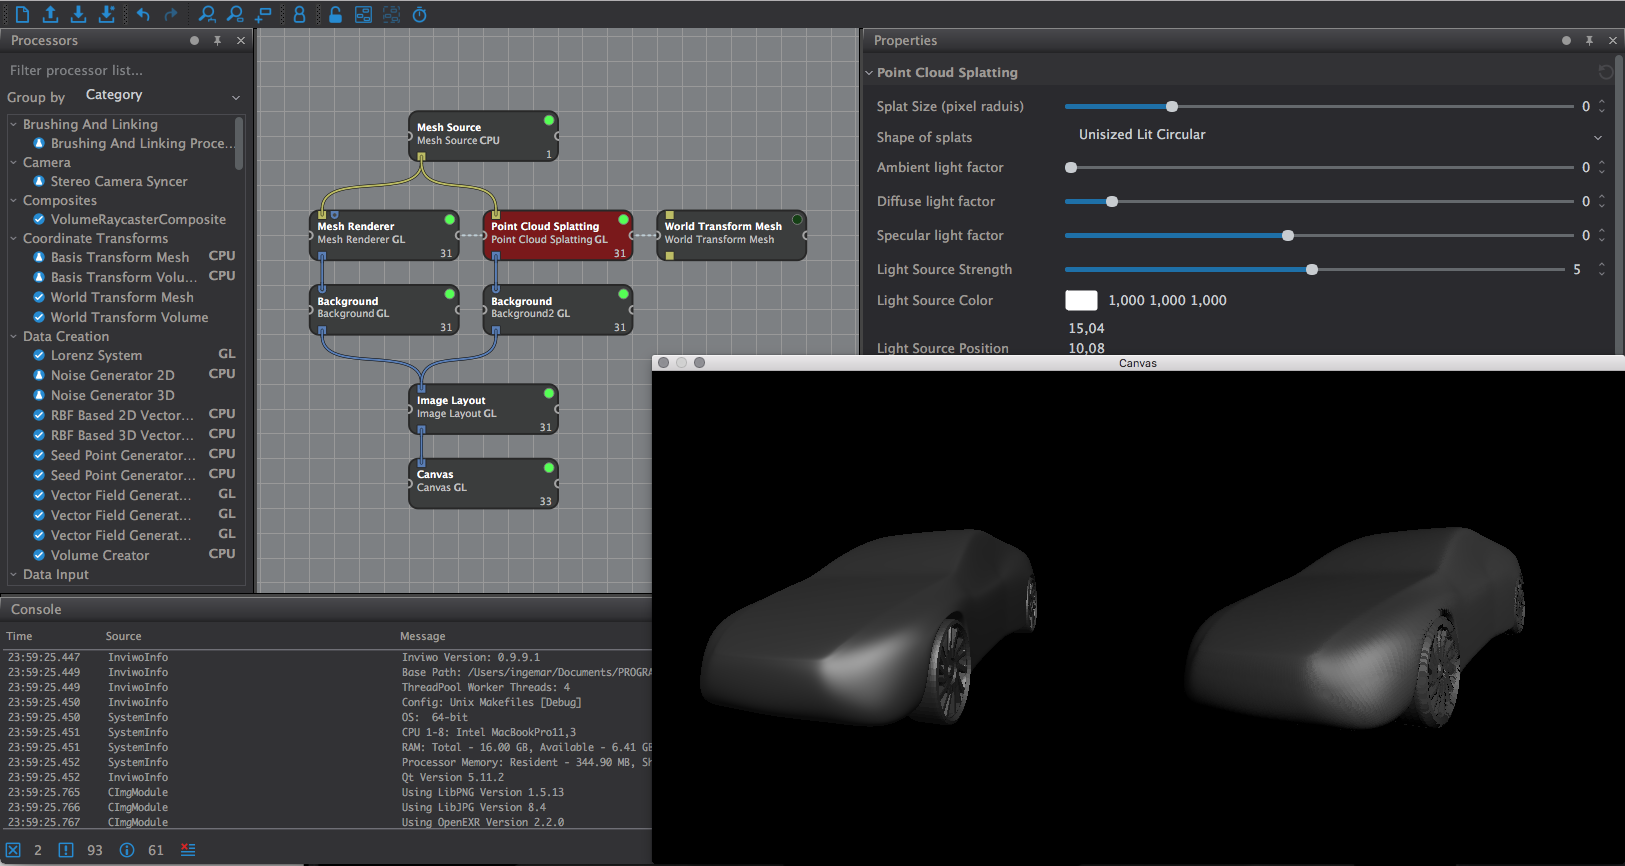
\includegraphics[width=.9\linewidth]{./images/ui.png}
\end{center}

\subsection*{Objective of this thesis}
\label{sec:orgac66f97}
\subsubsection*{Inviwo lacked:}
\label{sec:orgec9158e}
\begin{itemize}
\item A useful point splatting module.
\item A normal estimation processor for unorganized point clouds.
\end{itemize}

\subsubsection*{Research question}
\label{sec:org4673fc6}
How do different algorithms and datastructures for estimating normals in unorganized point clouds compare in terms of output quality and calculation time?

\subsubsection*{Goal}
\label{sec:org5673856}
\begin{itemize}
\item Implement a usable normal estimation and rendering solution for unorganized point clouds in Inviwo.
\end{itemize}

\subsubsection*{Why a new point splatting processor?}
\label{sec:orge61c2bb}
I wanted:
\begin{itemize}
\item Color-coded debug output of estimated normals.
\item Possible use of at least one light source.
\end{itemize}

\subsubsection*{Normal estimation evaluation}
\label{sec:orga795a9a}
\begin{itemize}
\item Output quality:
\begin{itemize}
\item Visual image inspection compared to references.
\item Numerical error distribution analysis.
\end{itemize}
\item Estimation running-time and resources
\begin{itemize}
\item Timing of each step in the estimation process.
\item Static analysis of memory usage.
\end{itemize}
\end{itemize}

\subsection*{Point splatting}
\label{sec:org059b169}
\subsubsection*{{\bfseries\sffamily TODO} Video}
\label{sec:orgf3e9d3b}
\subsubsection*{Reasons}
\label{sec:org5dca0a7}
\begin{itemize}
\item To few points to cover enough screen surface.
\item Down-sampling for increased calculation performance.
\end{itemize}

\subsubsection*{{\bfseries\sffamily TODO} How}
\label{sec:orgd0ff1ef}
Two images:
\begin{enumerate}
\item Only point
\item Point, plus four other points forming a splat.
\end{enumerate}

\subsubsection*{Variations}
\label{sec:orgc0b4141}
\begin{itemize}
\item Different shapes.
\item Placements offsets and angle.
\item Adaptive size to neighboring points.
\end{itemize}
\begin{center}
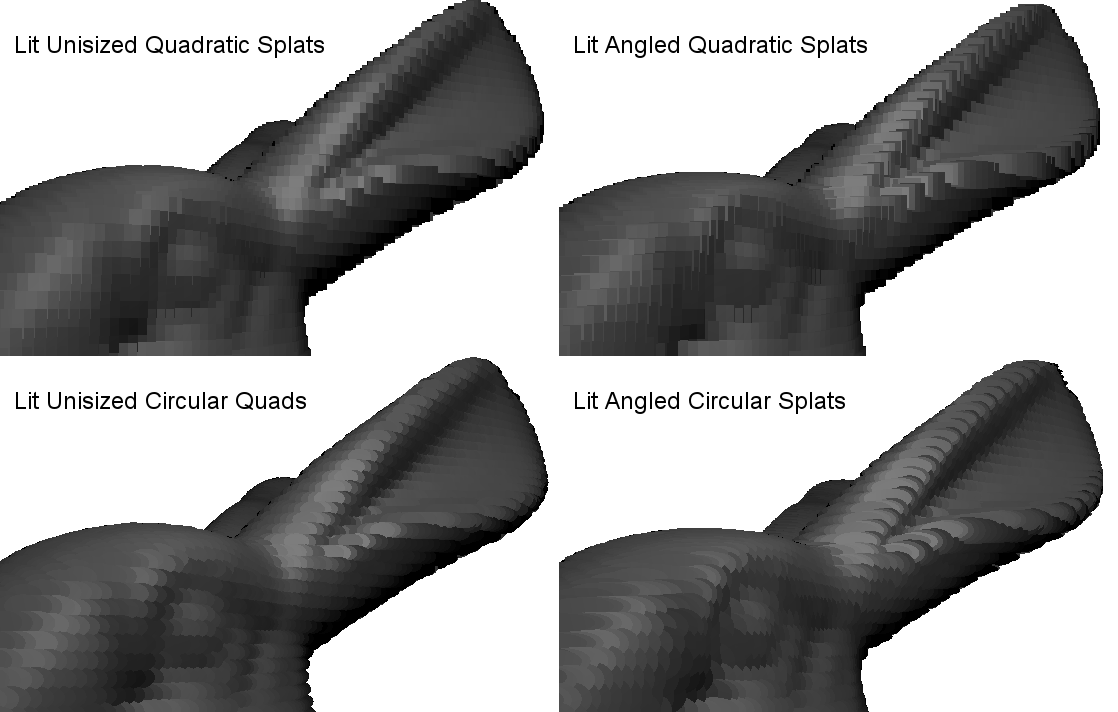
\includegraphics[width=.9\linewidth]{./images/Presentation_Splat_Variations.png}
\end{center}

\subsection*{Normal estimation}
\label{sec:orge678bd9}
\subsubsection*{What we see on screen}
\label{sec:org53a9bad}
A car:

\begin{center}
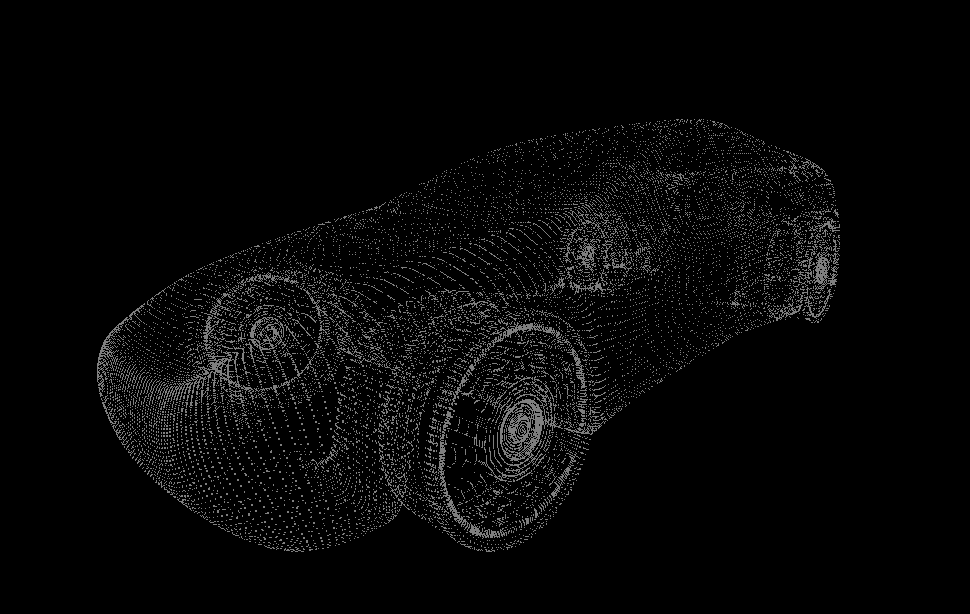
\includegraphics[width=.9\linewidth]{./images/Presentation_car_points.png}
\end{center}

\subsubsection*{What the computer see}
\label{sec:org18de491}
The same car:

\begin{center}
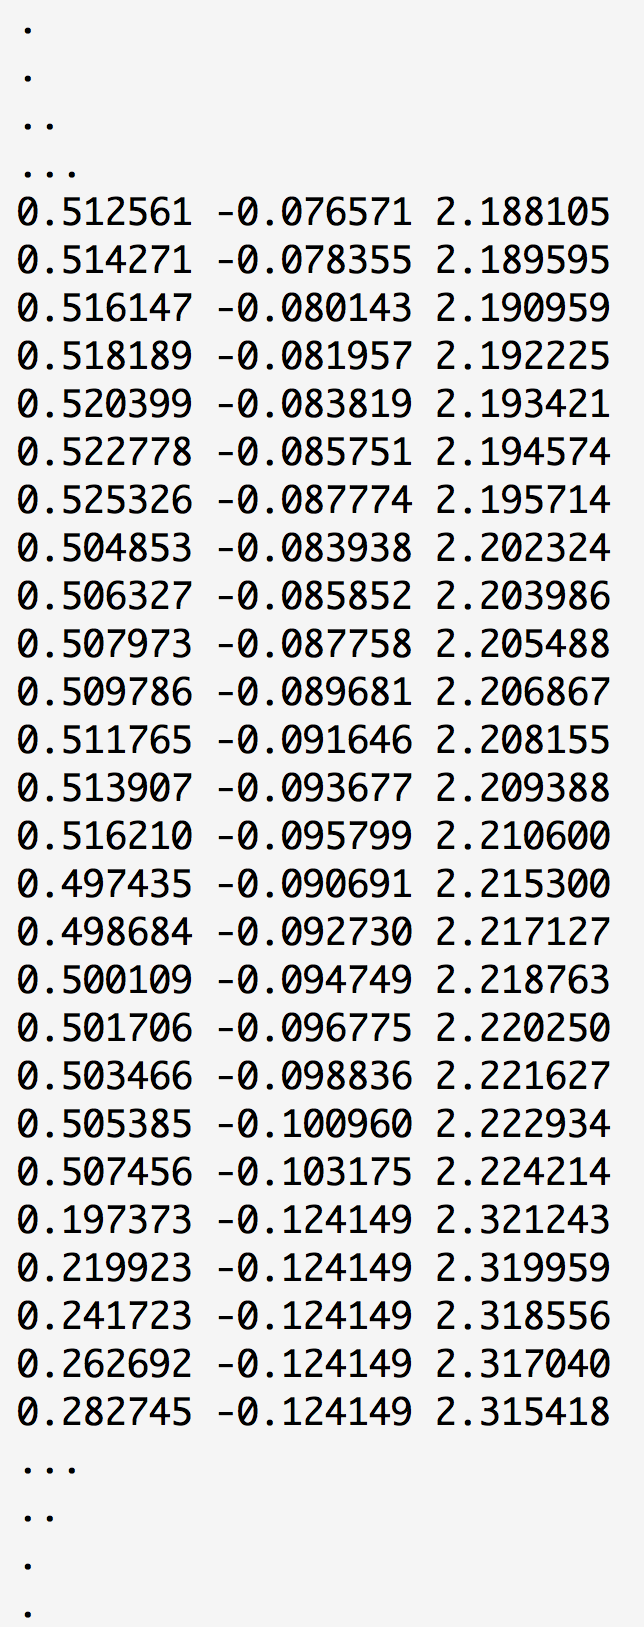
\includegraphics[width=.9\linewidth]{./images/Presentation_car_computervision.png}
\end{center}

\subsubsection*{Why estimate normals?}
\label{sec:org2b5ff82}
\begin{itemize}
\item Needed for proper light calculations.
\item Useful in computer vision and object recognition.
\end{itemize}

\begin{center}
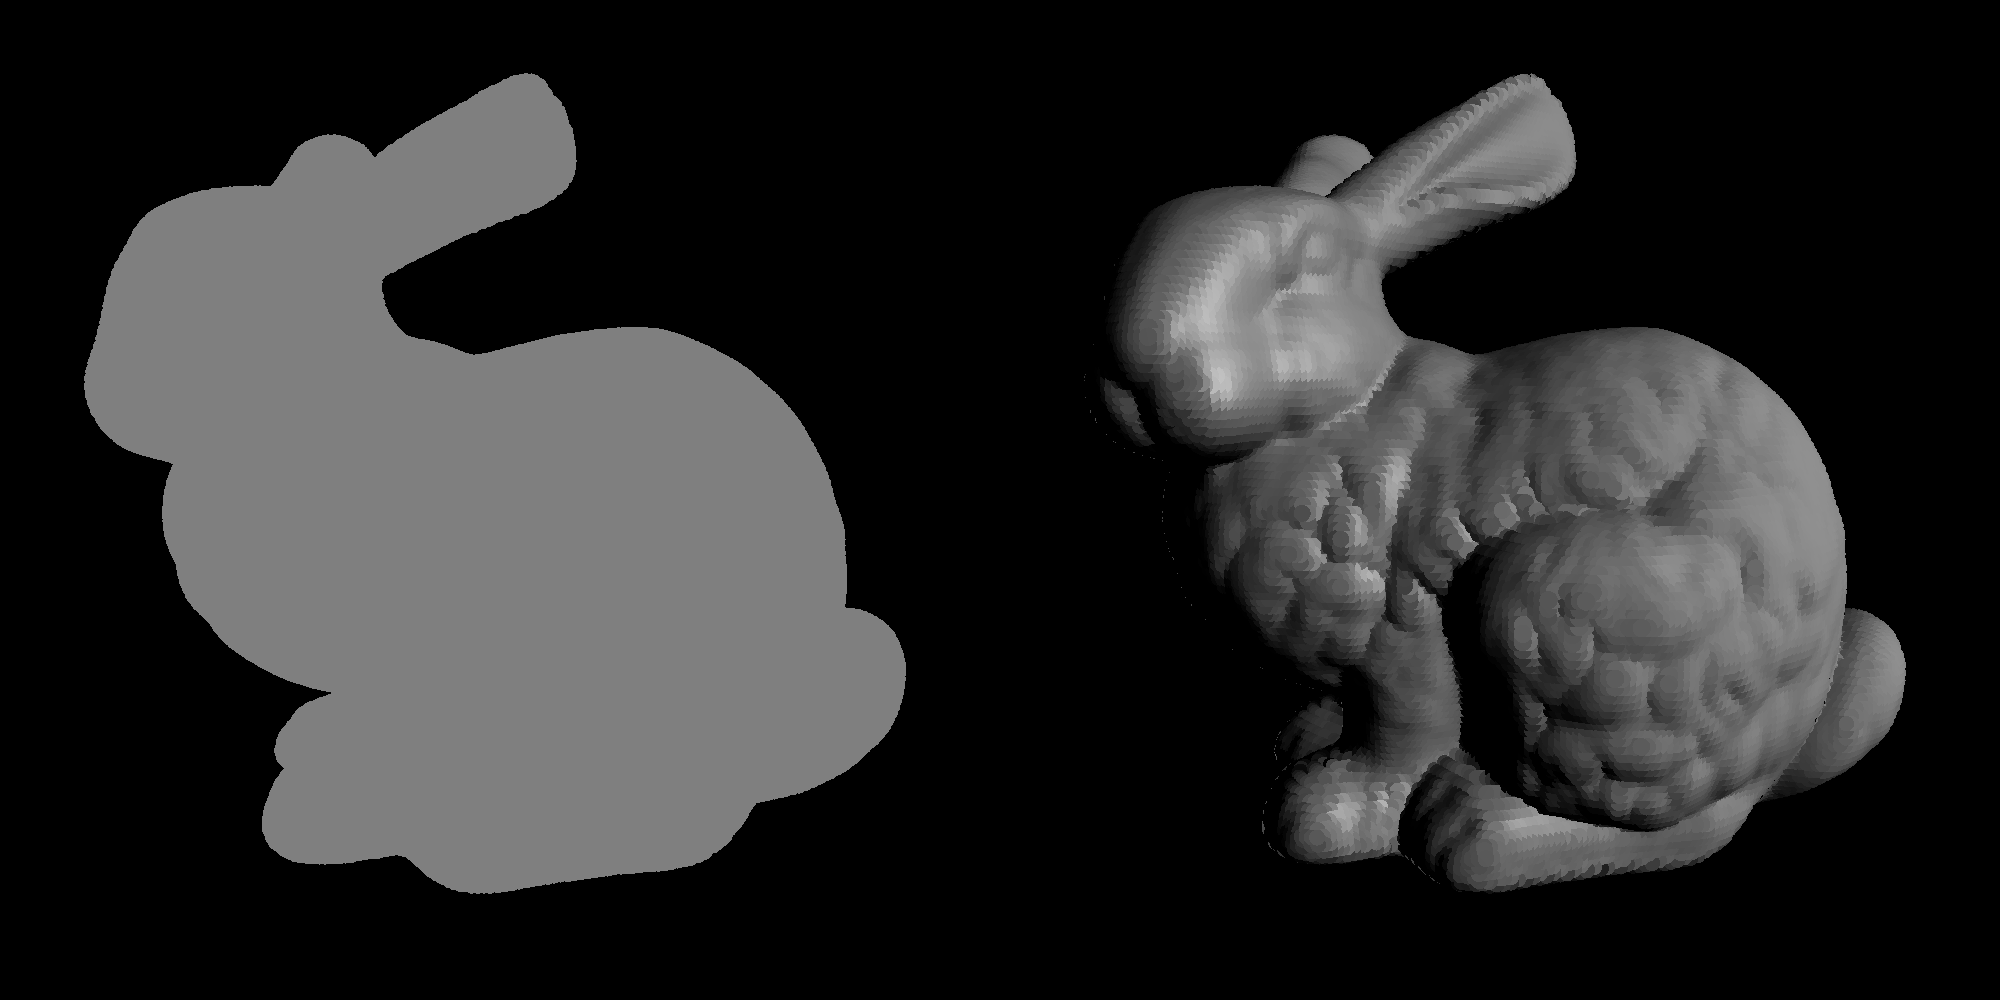
\includegraphics[width=.9\linewidth]{./images/Presentation_nonormals_normals.png}
\end{center}



\subsubsection*{Different approaches to normal estimation from neighborhoods}
\label{sec:org12bbb8b}
The two categories are:
\begin{enumerate}
\item Averaging methods.
\item Optimization methods.
\end{enumerate}

And the process can be described summarized as:
\begin{enumerate}
\item For each point \(\vec{p_i}\), find other nearby points \(E=[e_{i,1},e_{i,2},...,e_{i,k}]\).
\item Choose and use one of the methods above.
\end{enumerate}

\subsubsection*{Finding \(K\) point neighbors in an unorganized point cloud}
\label{sec:orgdc1a1fa}
\begin{itemize}
\item Both estimation categories utilize local neighborhoods.
\item Linear search is painfully slow (\(O(n^2*k)\))
\item Restructure the points into a tree structure. Which one?
\begin{itemize}
\item Oct-tree:
\begin{itemize}
\item Often used in game engines.
\item Fast creation.
\item Fast collision lookup, if the sub-tree searched from the root.
\end{itemize}
\item Equally spaced voxel grid:
\begin{itemize}
\item Intuitive neighboring voxel traversal.
\item However, possibly many empty voxels.
\end{itemize}
\item KD-tree:
\begin{itemize}
\item Balanced tree.
\item Slower initialization than the oct-tree.
\item Intuitive nearest neighbor querying.
\end{itemize}
\end{itemize}
\end{itemize}

\subsubsection*{KD-Tree}
\label{sec:org4d4eccd}
Worth remembering:
\begin{itemize}
\item The unorganized point cloud lacks any specific ordering.
\item Reordering points does not alter the visual output from the point splatting processor.
\end{itemize}

Building a 3D KD-tree from an unorganized point cloud \(P=[\vec{p_{start}},\vec{p_{start+1}},...,\vec{p_{end}}]\):
\begin{enumerate}
\item Find the median point \(p_m\) in a dimension \(d \in \left\{x,y,z\right\}\) among all points in \(P\).
\item Put all points with \(x_i < p_m\) before, and the rest after the median
\item Create two sub-trees (if there are any points left):
\begin{itemize}
\item \(t_{left}\) \(\rightarrow\) points \([\vec{p_{start}},...,\vec{p_{m-1}}]\).
\item \(t_{right}\) \(\rightarrow\) points \([\vec{p_{m+1}},...,\vec{p_{end}}]\).
\end{itemize}
\item Start over from \(1)\) for each sub-tree in another dimension.
\end{enumerate}

\subsubsection*{Nearest neighbor search}
\label{sec:org186f185}
\begin{itemize}
\item Two main types of neighborhoods:
\begin{itemize}
\item Fixed size.
\item All neighbors in a fixed radius.
\end{itemize}
\item The neighborhood search differs only in when to add-conditional.
\end{itemize}


\subsubsection*{Averaging methods}
\label{sec:org06ecc3c}

\subsubsection*{Variations}
\label{sec:orgbfea3dd}
\begin{itemize}
\item The number of triangles formed
\begin{itemize}
\item Fandisk (as in the video).
\item Complete triangulation of all neighbors.
\end{itemize}
\item Weighting the different triangles formed.
\begin{itemize}
\item Triangle edge length.
\item Triangle area.
\end{itemize}
\end{itemize}

\subsubsection*{Numerical methods (PCA)}
\label{sec:org7c40953}
Principal Component Analysis:
\begin{enumerate}
\item Find the nearest neighbours.
\item Create a covariance matrix \(M\) of the neighborhood.
\item Find the eigenvectors and eigenvalues of \(M\).
\item The smallest eigenvalue correspond to the neighborhood normal.
\end{enumerate}

\subsubsection*{Short standard image example in 2D}
\label{sec:orgab715d7}
\begin{center}
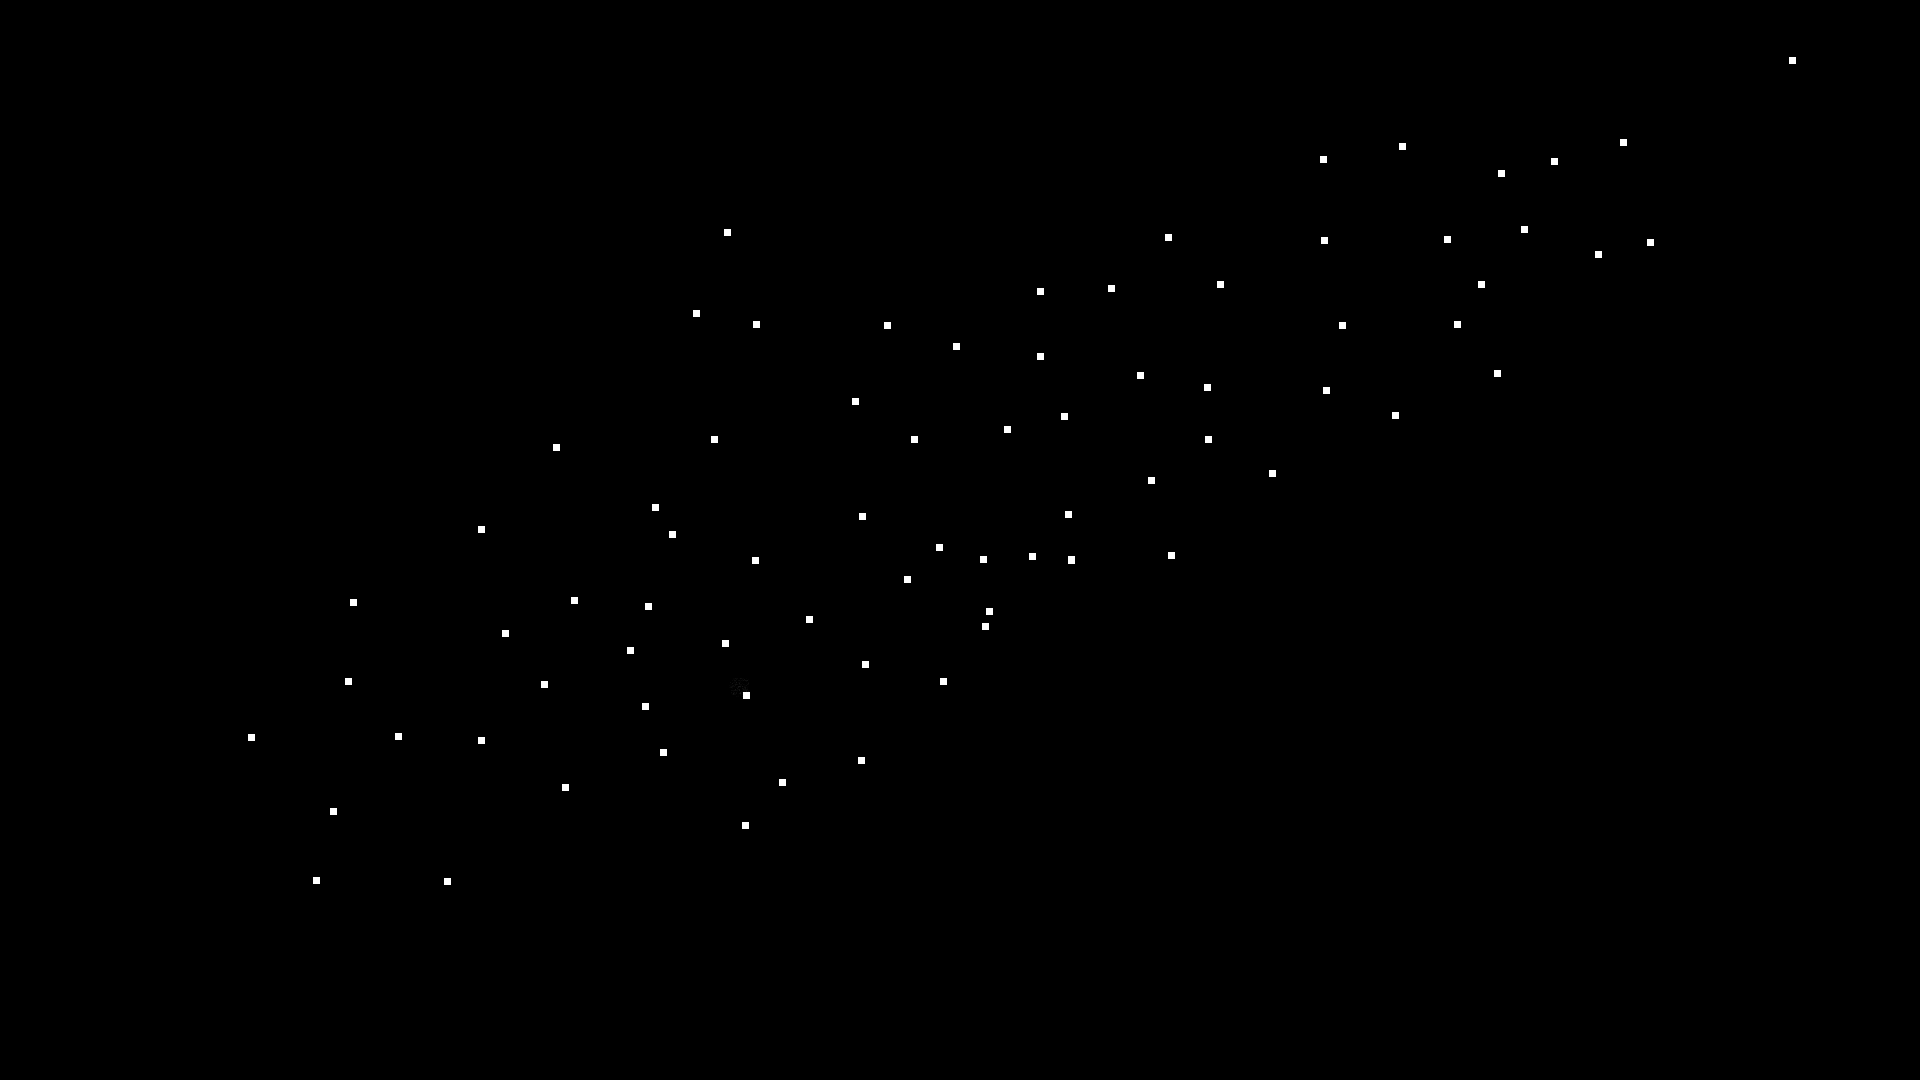
\includegraphics[width=.9\linewidth]{./images/pca_expl_img_points.png}
\end{center}

\begin{center}
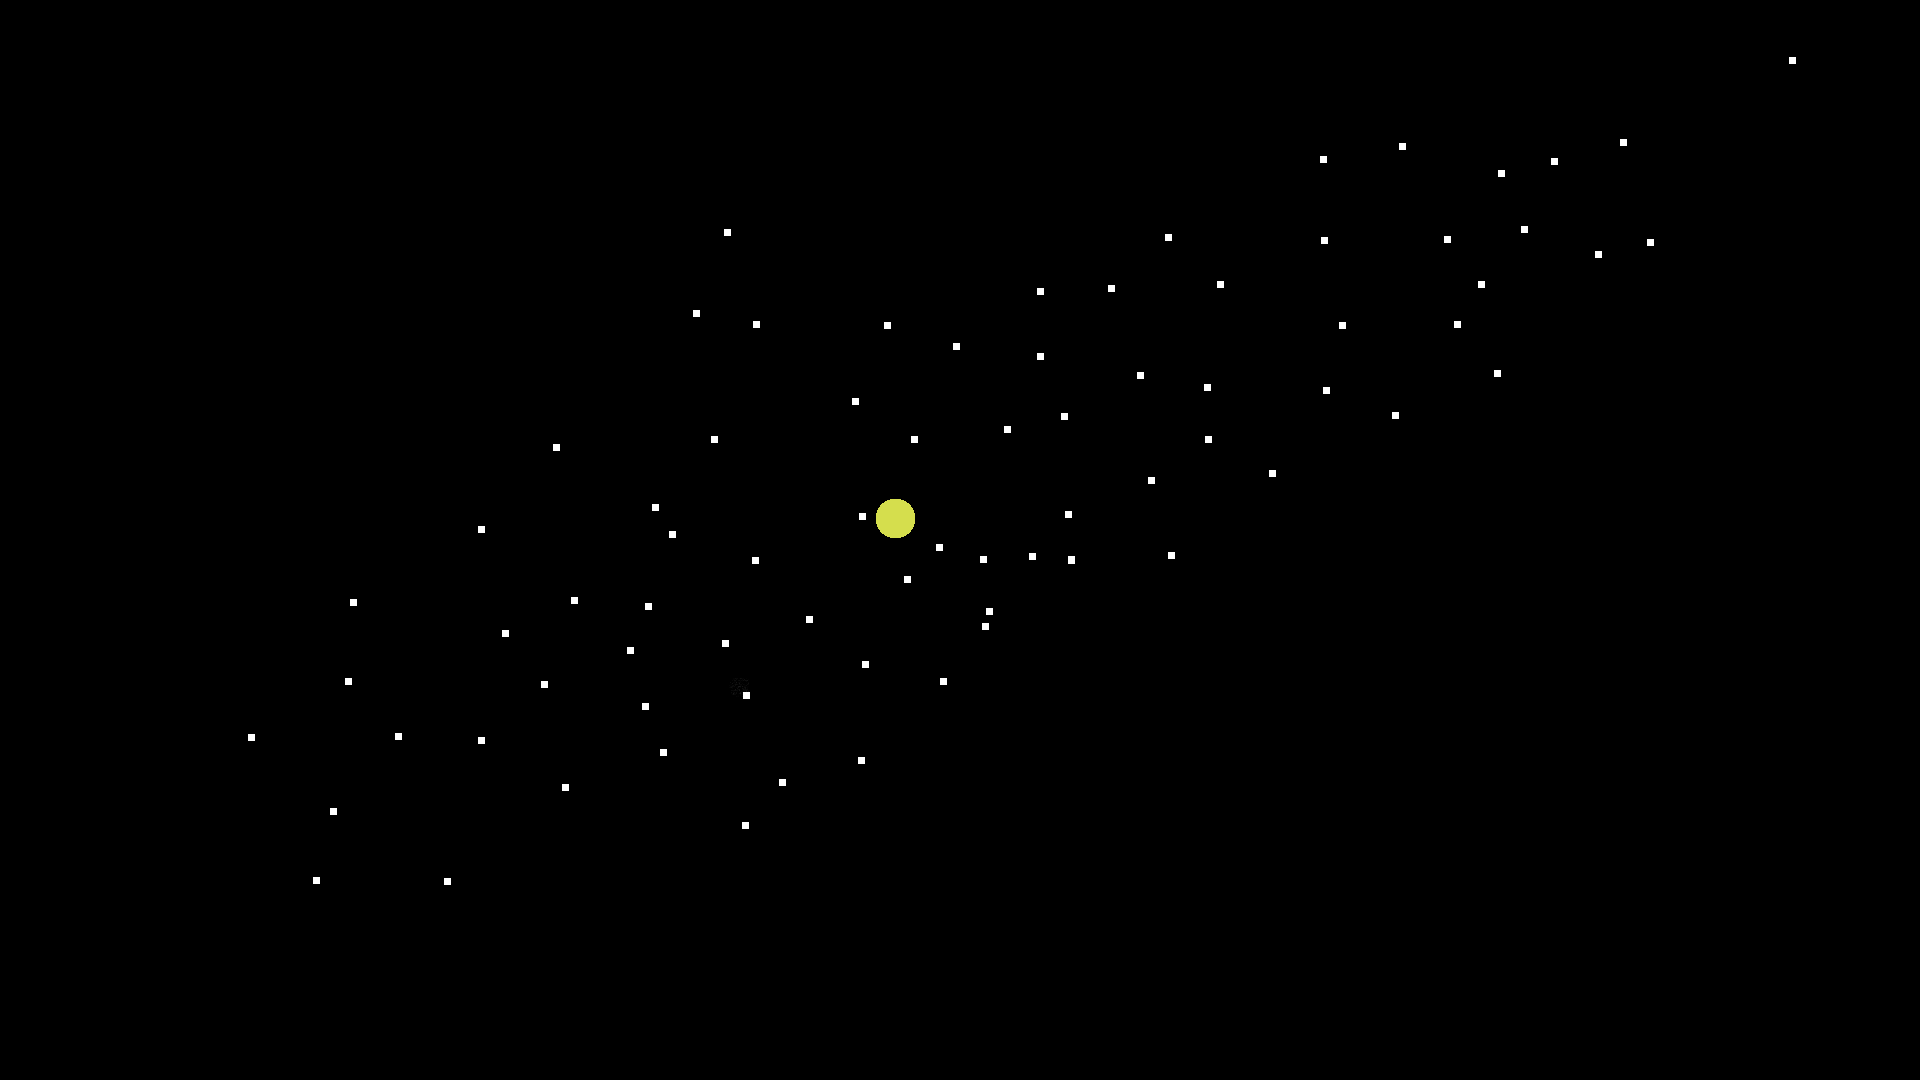
\includegraphics[width=.9\linewidth]{./images/pca_expl_img_points_mean.png}
\end{center}

\begin{center}
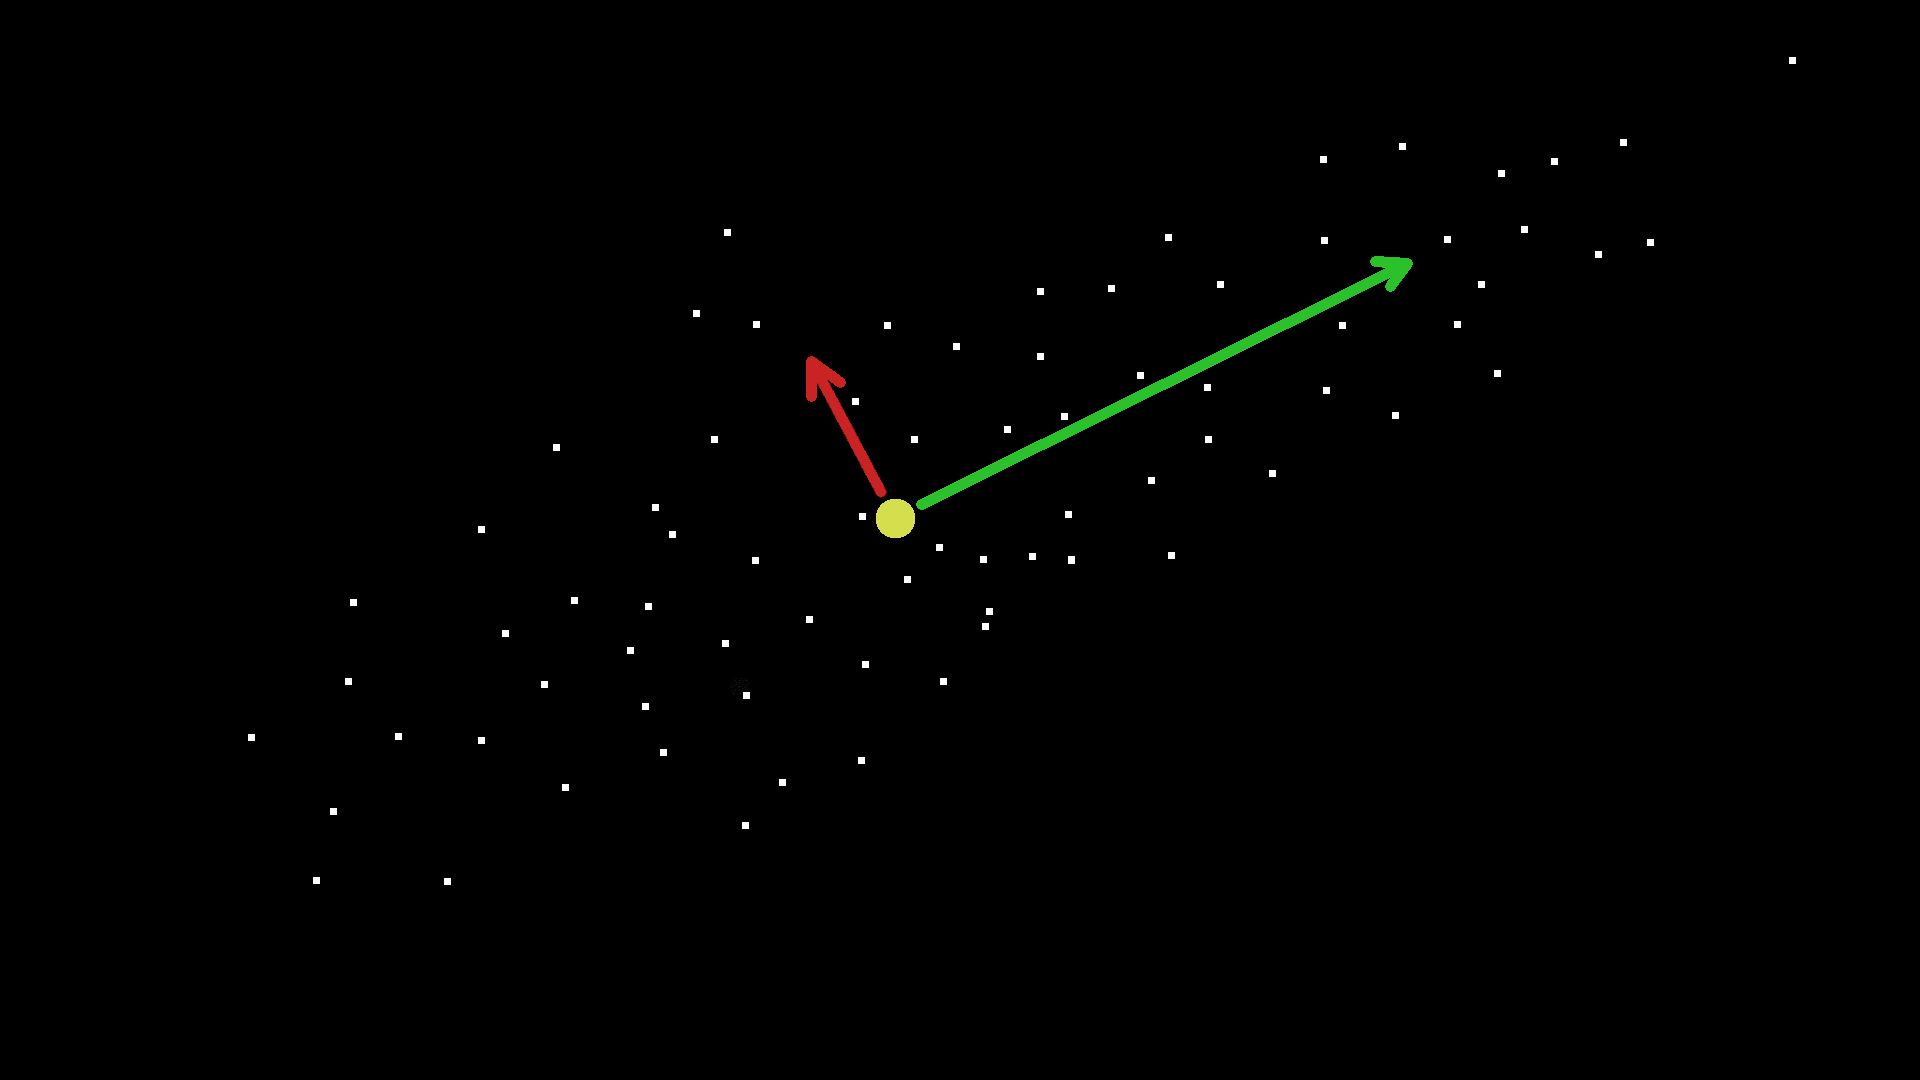
\includegraphics[width=.9\linewidth]{./images/pca_expl_img_points_mean_arrows.png}
\end{center}

\subsubsection*{When done on a 2D curve}
\label{sec:org6acdac4}

\begin{center}
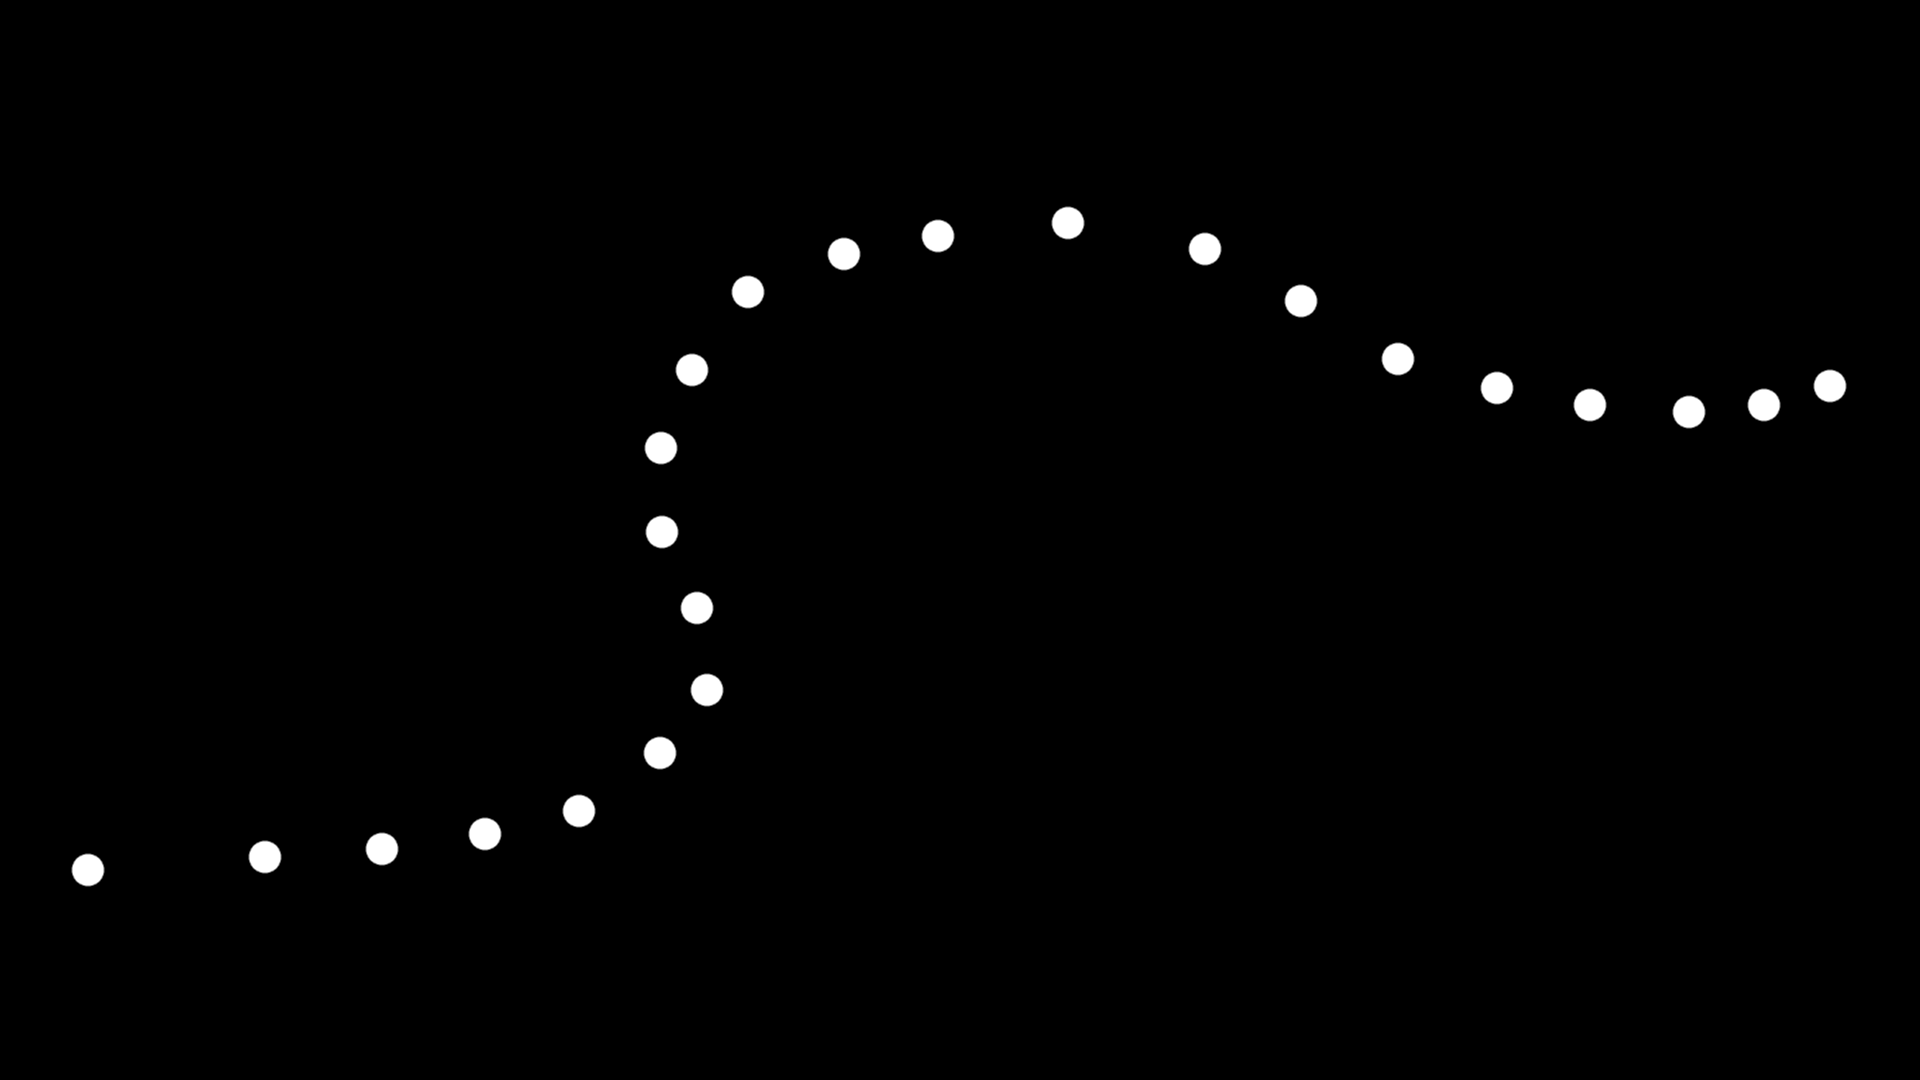
\includegraphics[width=.9\linewidth]{./images/pca_expl_line_points.png}
\end{center}

\begin{center}
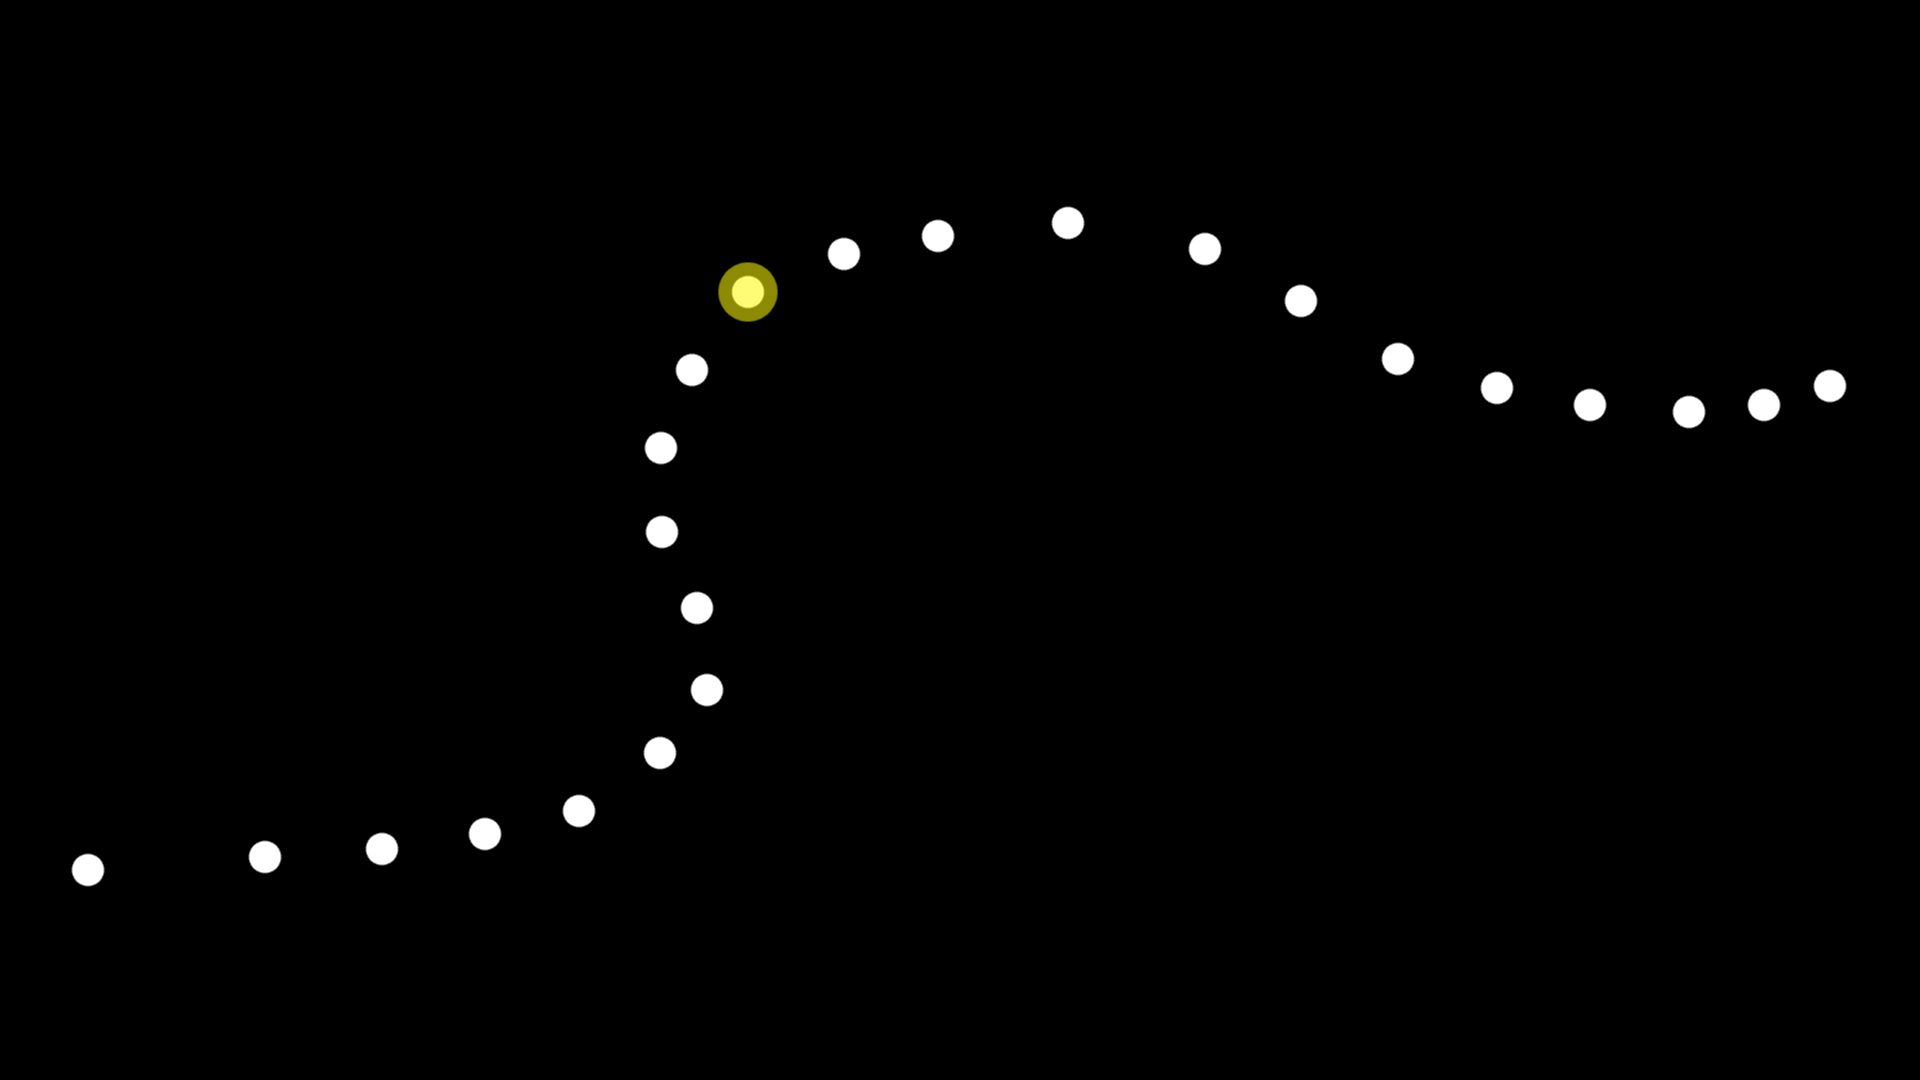
\includegraphics[width=.9\linewidth]{./images/pca_expl_line_points_seleceted.png}
\end{center}

\begin{center}
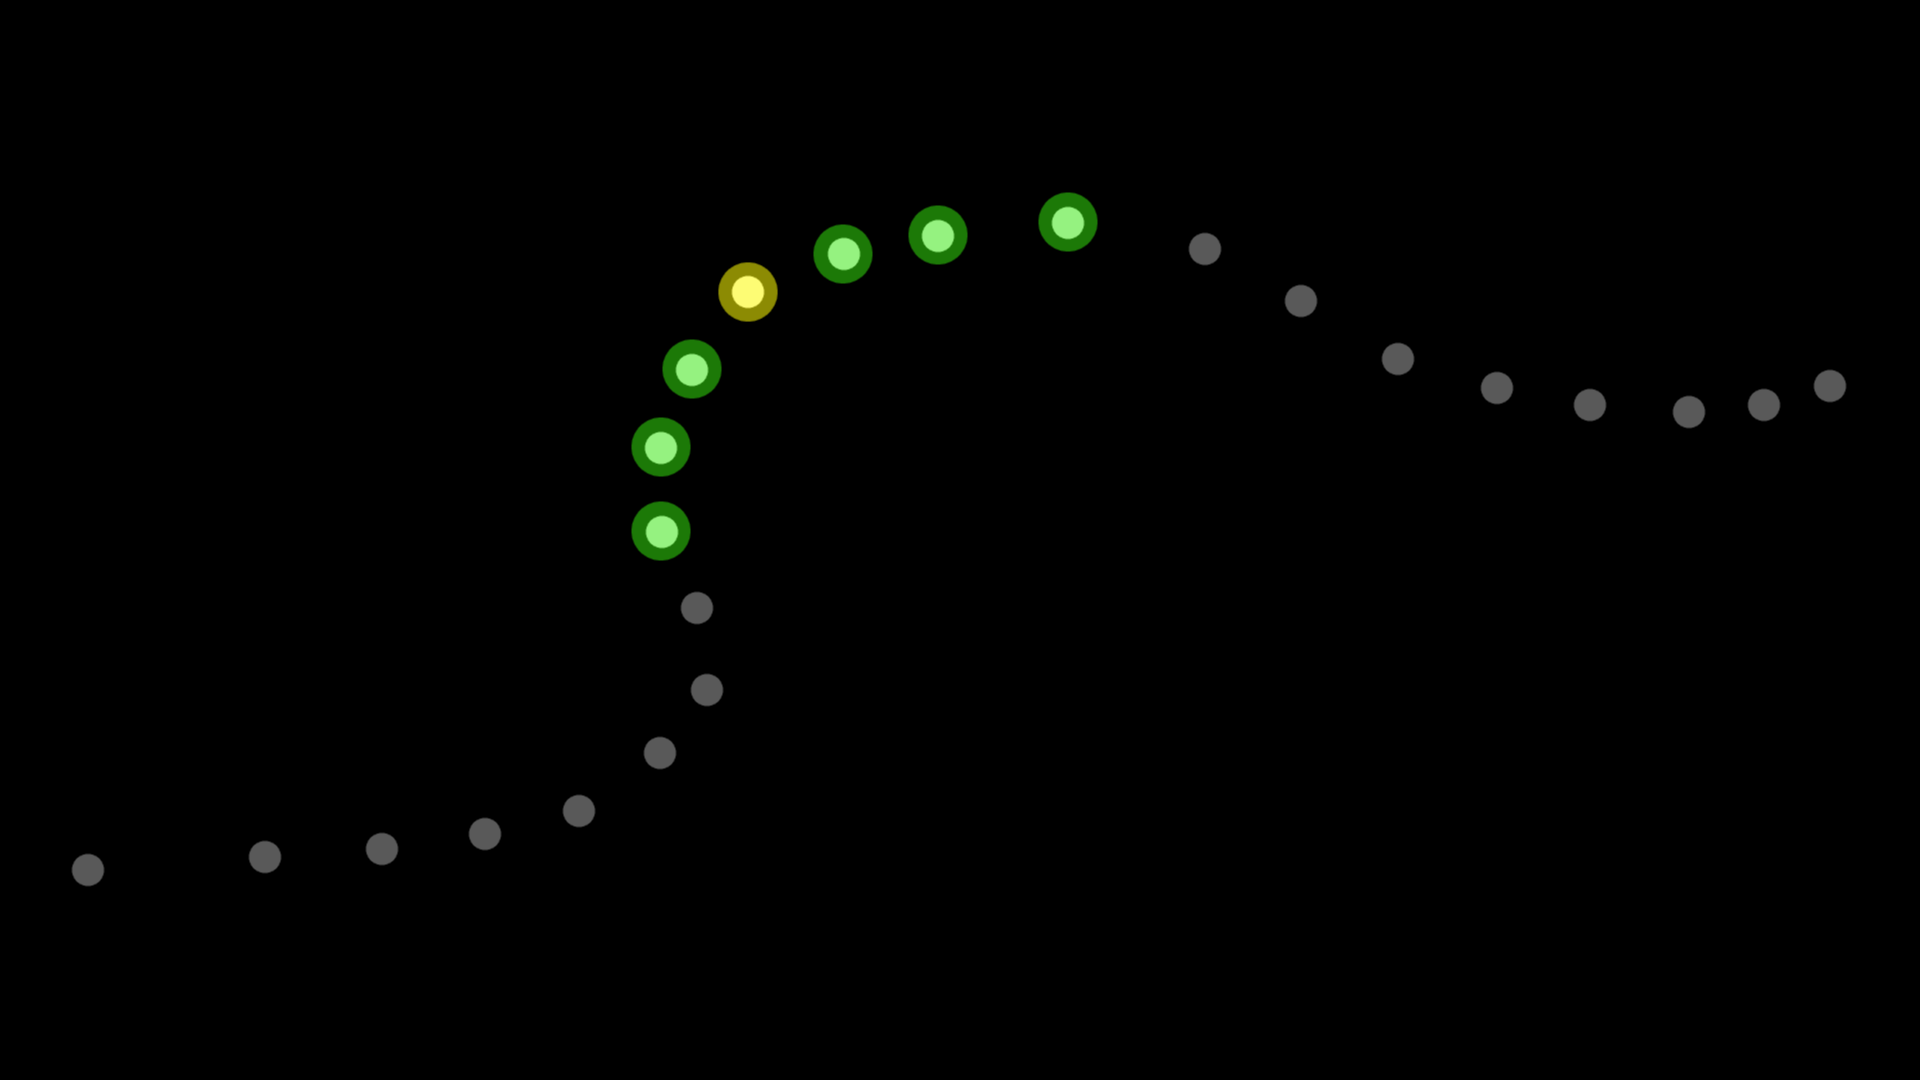
\includegraphics[width=.9\linewidth]{./images/pca_expl_line_points_seleceted_neighbors.png}
\end{center}

\begin{center}
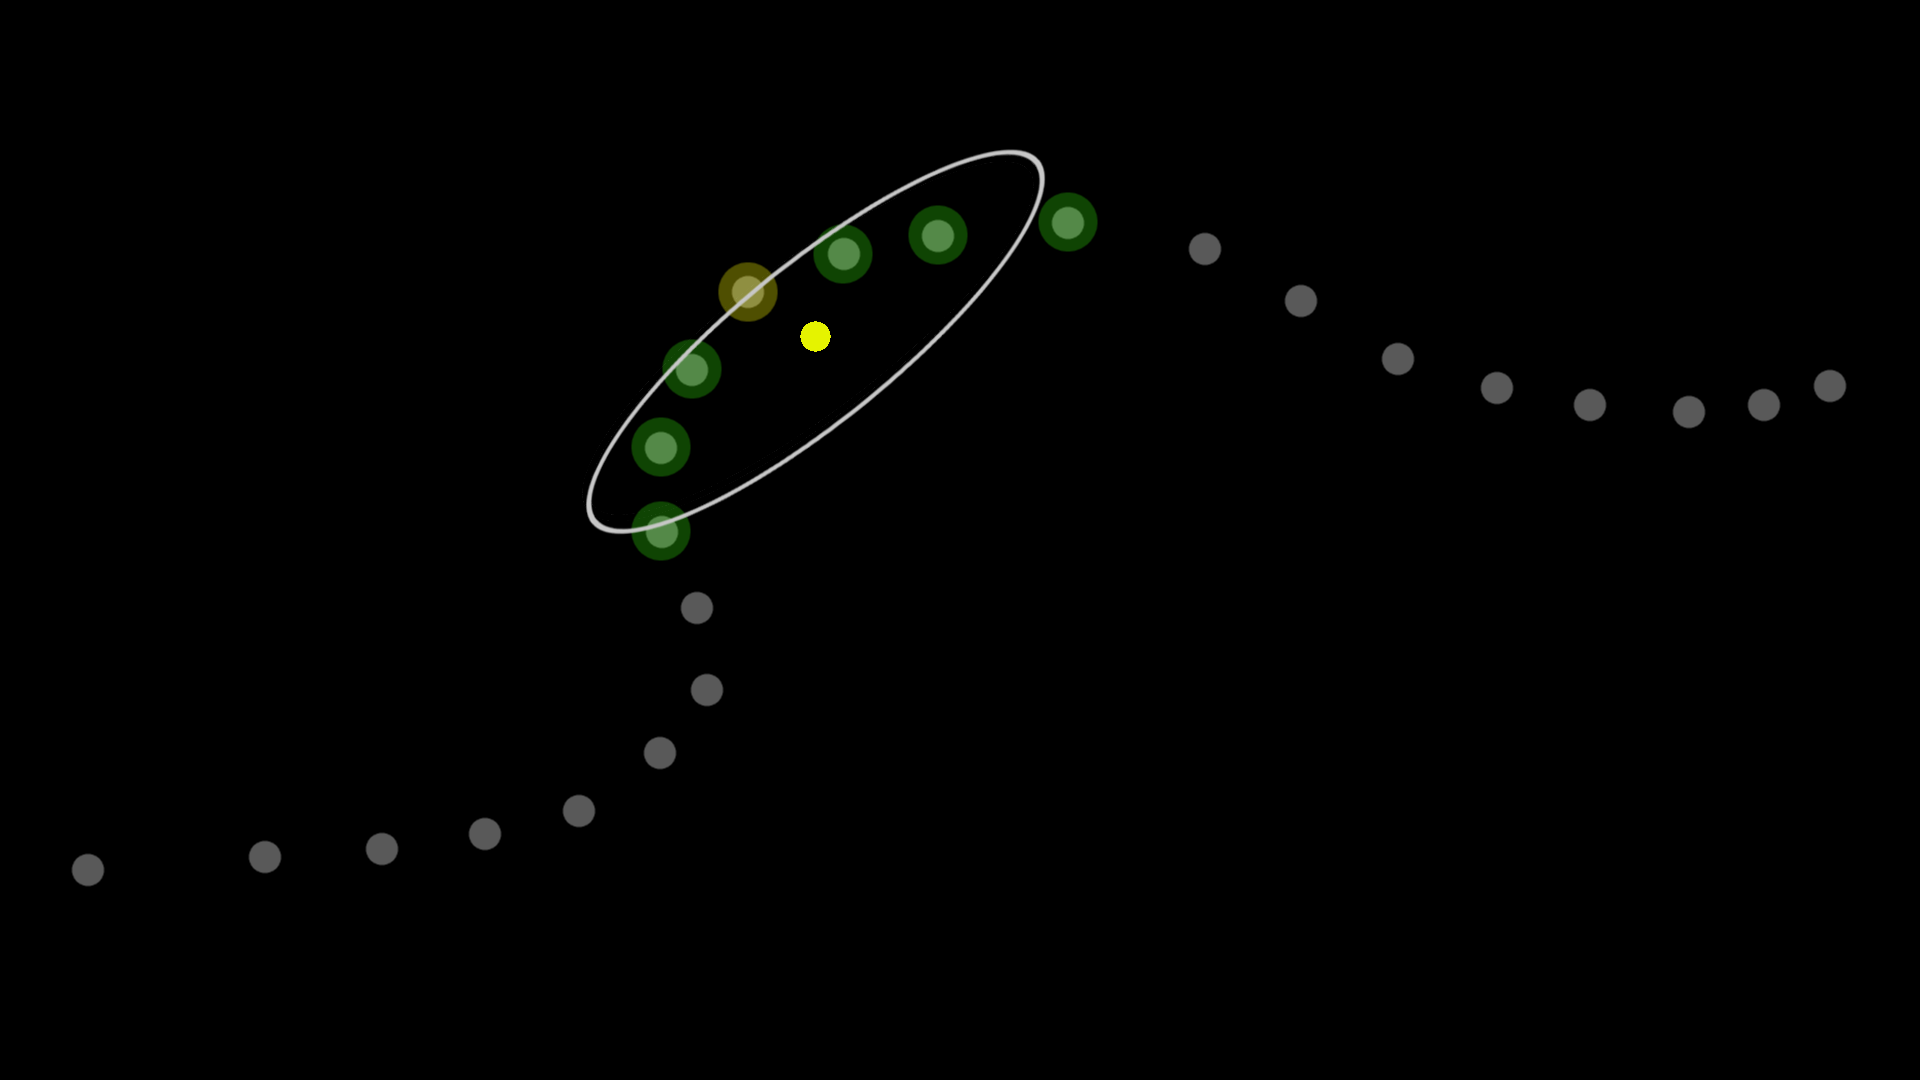
\includegraphics[width=.9\linewidth]{./images/pca_expl_line_points_seleceted_mean.png}
\end{center}

\begin{center}
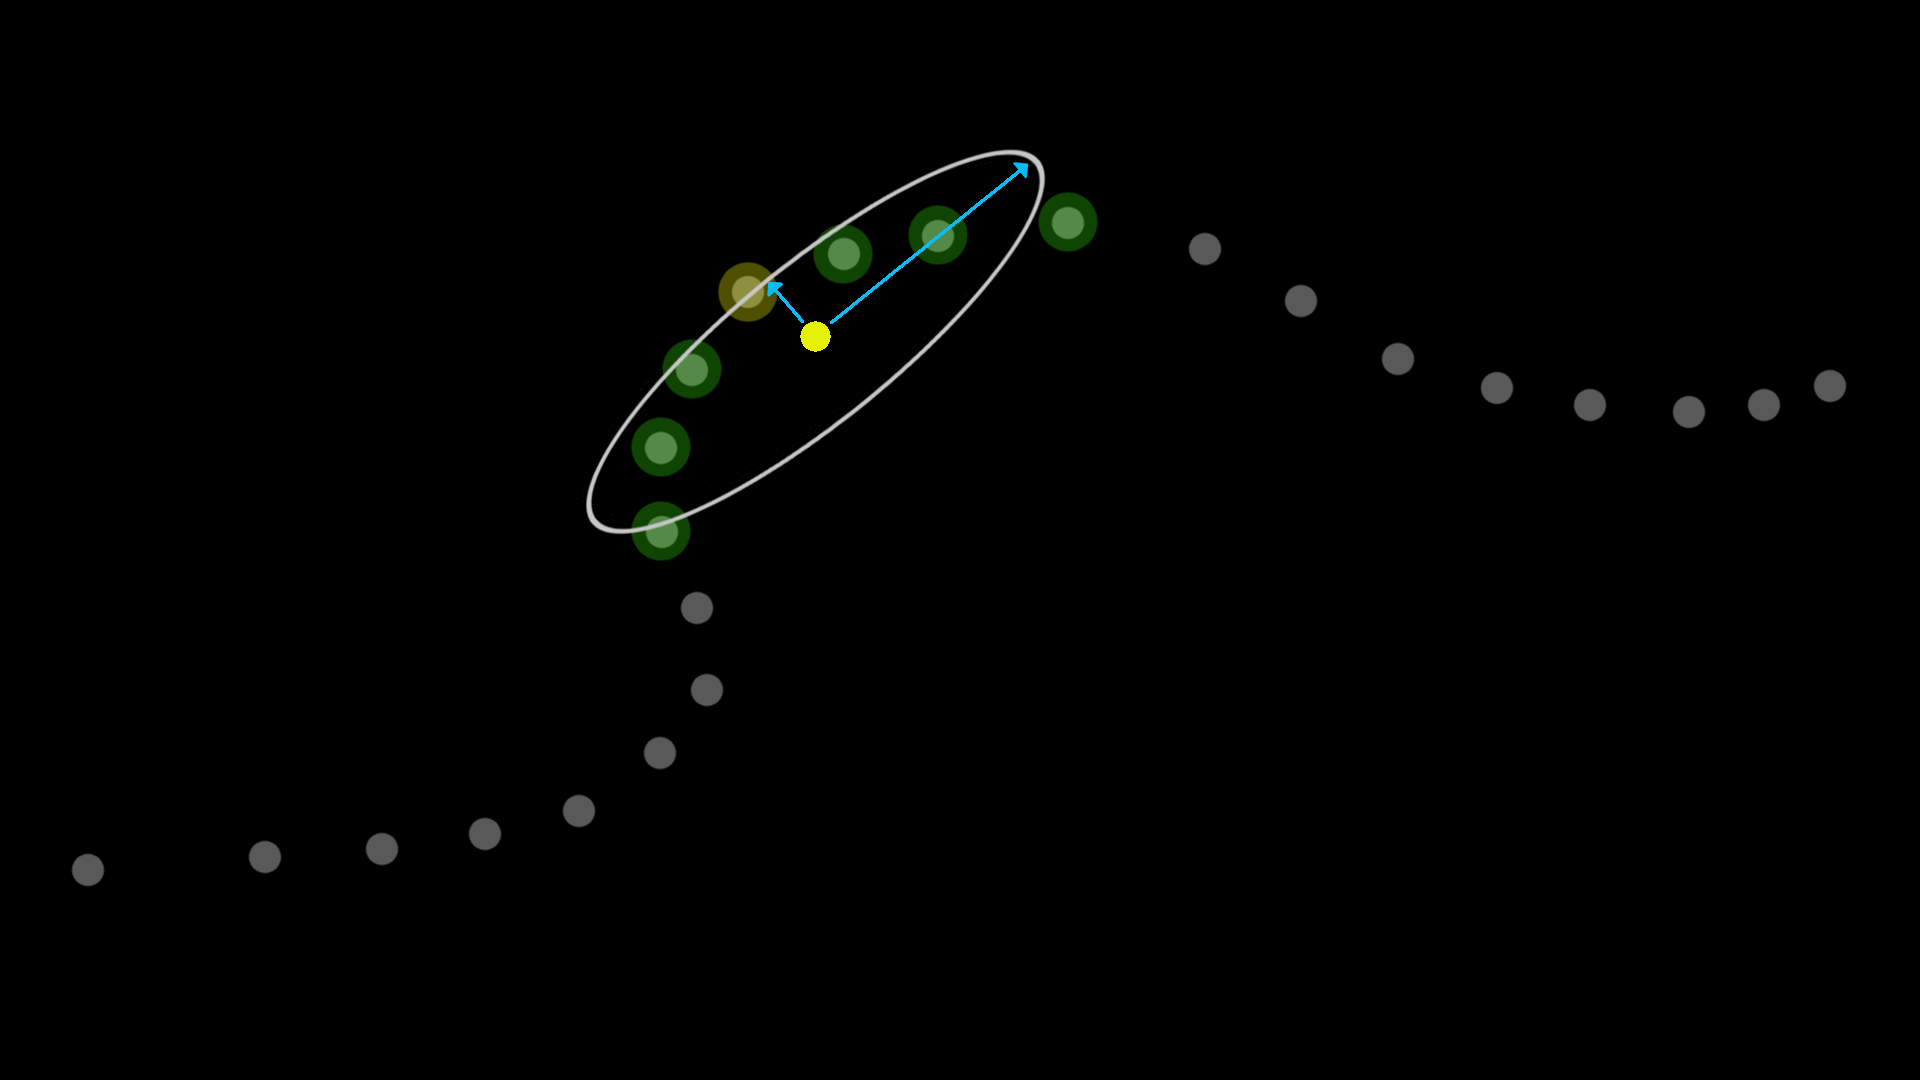
\includegraphics[width=.9\linewidth]{./images/pca_expl_line_points_seleceted_spread.png}
\end{center}

For a more explicit outline of the maths, see the report, section 2.3.2.
\end{document}
